\documentclass{aa}
\usepackage[varg]{txfonts}
\usepackage{float}
\usepackage{placeins}
\usepackage{nameref}
\usepackage{hyperref}
\usepackage{amsmath}
\usepackage{graphicx}
\usepackage{longtable}
\usepackage{comment}
\usepackage{booktabs}
\usepackage{longtable}
\usepackage{cuted}
% Croatian letter "dj"
\def\d   {{d $\mkern-14.3mu \mathchar'26 $}}

\title{Analysis of the Blazhko effect for field RR Lyrae stars}
\subtitle{using LINEAR and ZTF light curves}
\author{Ema Donev\inst{\ref{inst1}}
\and \v{Z}eljko Ivezi\'{c}\inst{\ref{inst2}}}

\institute{XV. Gymnasium (MIOC), Zagreb, Croatia, \email{emadonev@icloud.com}\label{inst1}
\and Department of Astronomy, University of Washington, Box 351580, Seattle, WA 98195, USA, \email{ivezic@uw.edu}\label{inst2}}
\date{October 2024}

\abstract{We analyzed the incidence and properties of stars that show evidence for amplitude, period, and
phase modulation (the so-called Blazhko Effect) in a sample of $\sim$3,000 field RR Lyrae stars with
LINEAR and ZTF light curve data. A preliminary subsample of about $\sim$240 stars was selected
using various light curve statistics, and then $\sim$140 stars were confirmed visually as displaying
the Blazhko effect. Although close to 8,000 Blazhko stars were discovered in the Galactic bulge
and LMC/SMC by the OGLE-III survey, only about 200 stars have been reported in all field RR Lyrae stars studies to date.}

\keywords{Variable stars --- RR Lyrae stars --- Blazhko Effect}

\begin{document}
\maketitle

\section{Introduction\label{sec:intro}}

RR Lyrae stars are pulsating variable stars with periods in the range of 3--30 hours and large amplitudes
that increase towards blue optical bands (e.g., in the SDSS $g$ band from 0.2 mag to 1.5 mag;
\citealt{2010ApJ...708..717S}). For comprehensive reviews of RR Lyrae stars, we refer the reader to \cite{1995CAS....27.....S} and \cite{2009Ap&SS.320..261C}.

They often exhibit amplitude, period, and phase modulation, or the so-called Blazhko effect (hereafter,
``Blazhko stars''). For examples of well-sampled observed light curves showing the Blazhko effect, see,  e.g., Kepler
data shown in Figures 1 and 2 from \cite{2010MNRAS.409.1585B}. The effect has been known for a long time \citep{1907AN....175..325B}, but its detailed observational
properties and theoretical explanation of its causes remain elusive \cite{2009AIPC.1170..261K}.

References to various proposed models for the mysterious Blazhko effect and main
reasons why they fail to explain observations are summarized in \cite{2016CoKon.105...61K}. 

A part of the reason for the incomplete observational description of the Blazhko effect is difficulties in discovering a large number 
of Blazhko stars due to temporal baselines that are too short and insufficient number of observations per object
\citep{2016CoKon.105...61K,2022ApJS..258....4H}. With the advent of modern sky surveys, several studies
reported large increases in the number of known Blazhko stars, starting with a sample of about 700 Blazhko
stars discovered by the MACHO survey towards LMC \citep{2003ApJ...598..597A} and about 500 Blazhko stars
discovered by the OGLE-II survey towards the Galactic bulge \citep{2003AcA....53..307M}. 
Most recently,  about 4,000 Blazhko stars were discovered in the Large and Small Magellanic Clouds
\citep{2009AcA....59....1S, 2010AcA....60..165S}, and an additional $\sim$3,500 stars were discovered in the
Galactic bulge \citep{2011AcA....61....1S}, both by the OGLE-III survey. Nevertheless, discovering the Blazhko
effect in field RR Lyrae stars that are spread over the entire sky remains a much harder problem: only about
200 Blazhko stars in total from all the studies of field RR Lyrae stars have been reported so far (see Table 1
in \citealt{2016CoKon.105...61K}). 

Here, we report the results of a search for the Blazhko effect in a sample of $\sim$3,000 field RR Lyrae stars with
LINEAR and ZTF light curve data. A preliminary subsample of about $\sim$240 stars was selected using various
light curve statistics, and then $\sim$140 stars were confirmed visually as displaying the Blazhko effect. This new
sample greatly increases the number of known field RR Lyrae stars that exhibit the Blazhko effect. In \S\ref{sec:analysis}
we describe our datasets and analysis methodology, and in \S\ref{sec:results} we present our analysis results. 
Our main results are summarized and discussed in \S\ref{sec:discussion}.

\section{Data Description and Analysis Methodology}\label{sec:analysis}
Our chosen surveys for this project were the LINEAR asteroid survey and, subsequently, the ZTF survey, 
from which we selected the corresponding LINEAR stars. The ZTF survey monitored the sky $\sim$10 years after LINEAR, providing a unique opportunity for analysis. In this work, we used the programming language Python. The entirety of the code can be found on GitHub\footnote{\url{https://github.com/emadonev/var_stars}}.  


\subsection{LINEAR Dataset}

The properties of the LINEAR asteroid survey and its photometric re-calibration based on SDSS data are discussed in \cite{2011AJ....142..190S}.
Briefly, the LINEAR survey covered about 10,000 deg$^2$ of the northern sky in white light (no filters were used, see Figure 1 in \citealt{2011AJ....142..190S}),
with photometric errors ranging from $\sim$0.03 mag at an equivalent SDSS magnitude of $r=15$ to 0.20 mag at $r\sim18$. Light curves used
in this work include, on average, 270 data points collected better between December 2002 and March 2008.
 
A sample of 7,010 periodic variable stars with $r<17$ discovered in LINEAR data was robustly classified by \cite{2013AJ....146..101P}, including
about $\sim$3,000 field RR Lyrae stars detected to distances of about 30 kpc \citep{2013AJ....146...21S} of both ab and c type. The sample used in this work contains 2196 ab-type and 745 c-type RR Lyrae, selected using classifications and the {\it gi} color index from \cite{2013AJ....146..101P}.
The LINEAR light curves, completed with IDs, equatorial coordinates, and other data, were accessed using the astroML Python module.

\subsection{ZTF Dataset}

The Zwicky Transient Facility (ZTF) is an optical time-domain survey that uses the Palomar 48-inch Schmidt telescope
and a camera with 47 deg$^2$ field of view \citep{2019PASP..131a8002B}. The data analyzed here was obtained with
SDSS-like $g$, $r$, and $i$ band filters. Light curves for objects in common with the LINEAR RR Lyrae sample typically
have smaller random photometric errors than LINEAR light curves because ZTF data are deeper (compared to LINEAR,
ZTF data have about 2-3 magnitudes fainter  $5\sigma$ depth).

The ZTF dataset for this project was created by selecting ZTF IDs with matching equatorial coordinates to a corresponding LINEAR ID of an RR Lyrae star. This process used the {\it ztfquery} function, which searched the coordinates database within a r$\sim$3. Our sample consisted of 2857 stars. 

\subsection{Analysis of RR Lyrae stars}

We used several methods and tools to analyze our RR Lyrae star sample thoroughly. Previous research has shown that the Blazhko effect presents itself as a modulation of period or amplitude, or it is visible in the star's periodogram. In the following section, we describe methods for such analysis.

The periodic shape change of light curves for Blazhko stars is equivalent to periodic phase and amplitude changes of the
harmonics that make up the light curve. This work used the Lomb-Scargle method for period calculation and periodogram analysis. By finding specific harmonics that create the final shape of the light curve and representing their power of fit using a periodogram, we can find a potential {\it blazhko frequency}.

Comparing the Blazhko effect as a {\it blazhko frequency} interfering with the intrinsic frequency of pulsation of an RR Lyrae, it is observed that modulation of either period or amplitude arises. The effect is known as \textbf{interference beats}, described by the equation below:
\begin{equation*}
    y(t) = 2 \, cos(2\pi \ \Delta f) \, sin(2\pi \ f_{avg})
\end{equation*}
Where $\Delta f$ is the difference between the primary and Blazhko frequency, and $f_{avg}$ is the average between the two frequencies.

A periodogram from a Blazhko star would contain a central peak with two equally distant local peaks at frequencies $f_-$ and $f_+$, with $f_- < f_0 < f_+$, where $f_0$ is the frequency of the main pulsation. The sideband peaks can be highly asymmetric
\cite{2003ApJ...598..597A}. Observing periodograms can sometimes be much more complex \cite{2007MNRAS.377.1263S}.  

For this project, we created an algorithm that searches for an interfering \textit{blazhko frequency} by folding the periodogram through the main peak and comparing if the folded peaks were statistically more significant than the background noise. The algorithm utilized the increased SNR due to the multiplication of peaks. It also eliminated stars with a yearly alias.

The Blazhko period, calculated if the algorithm finds the Blazhko frequency, is defined as
\begin{equation*}
P_{BL} = |f_{-,+} - f_0|^{-1},
\end{equation*}
where $f_{-,+}$ means the Blazhko sideband frequency with a higher amplitude is chosen. 

The observed Blazhko periods range from 3 to 3,000 days, and Blazhko amplitudes range from 0.01 mag to about 0.3 mag \citep{2007MNRAS.377.1263S}. In this work, we select a smaller Blazhko range due to the range of our data.
\begin{figure}
  \centering
  \resizebox{\hsize}{!}{\includegraphics[width=14cm]{periodogram.png}}
       \caption{Comparison of theoretical interference beats for a simulated light curve and real periodogram data from LINEAR and ZTF datasets.}
       \label{fig:periodogram}
  \end{figure}

  Fig \ref{fig:periodogram} compares the theoretical periodogram produced by interference beats with our algorithm's periodogram, signifying that local Blazhko peaks are present in real data.

The Blazhko effect most commonly presents as a modulation of amplitude, period, or both. 
We phased the light curves, calculated their fit, and $\chi^2$ value was also calculated. The $\chi^2$ value gives a quantitative representation of \textit{"goodness of fit"}, which shows us if modulation is present. Fig \ref{fig:lc_pair} shows an example star with LINEAR and ZTF phased light curves, along with their {\it fits}. 

\begin{figure}[ht]
  \centering
  \resizebox{\hsize}{!}{\includegraphics[width=14cm]{lc_pair.png}}
       \caption{Comparison of theoretical interference beats for a simulated light curve and real periodogram data from LINEAR and ZTF datasets.}
       \label{fig:lc_pair}
  \end{figure}

  \subsection{Searching for the Blazhko Effect}

For efficient and robust analysis, another algorithm was developed to select viable Blazhko candidates to be visually analyzed. 
The algorithm removed all stars with unrealistic data or insufficient data points (250 for LINEAR and 40 for ZTF). 
Then, it removed stars whose \textit{blazhko peak} was a yearly/daily alias, whose relative strength of peaks was below 0.05, and whose significance was below 5—their Blazhko period had to be between 30 and 325 days. 
The selection of stars based on the period difference (difference between LINEAR and ZTF period, divided by the mean period), amplitude, and the $\chi^2$ value was made using a scoring mechanism. 
Based on the distribution of period differences and $\chi^2$ values, it was determined for LINEAR that $1.8<\chi^2<3.0$ was worth 2 and $\chi^2>3.0$ worth 3 points, while for ZTF $2.0<\chi^2<4.0$ and $\chi^2>4.0$ were the limits. If both $\chi^2$ parameters were satisfied, it was worth 4 or 6 points, respective of the limits. 
The limits of the period difference were $0.00002 < dP < 0.00005$ worth 2, and $dP > 0.00005$ worth 4 points. Finally, $0.05 < ample < 0.15$ was worth one, and $0.15 < ample < 2.00$ was worth 2 points. 
A star could score a maximum of 12 points or be directly selected via its \textit{blazhko frequency}.
A smaller sample of 239 Blazhko candidates was selected. Visual analysis was separated into five categories: LINEAR or ZTF \textit{blazhko frequency}, LINEAR or ZTF $\chi^2$ value, and none of the above. 

Firstly, the shape and noisiness of the phased light curves were examined. 
If it was deemed that the light curve was precise enough, and if the phase contained different shapes. 
Fig \ref{fig:phase1} shows the first phase of visual analysis, where the ZTF fit shows signs of the Blazhko effect.

Secondly, the correctness of the algorithm in recognizing the \textit{blazhko frequency} was examined. Fig \ref{fig:phase2} shows an example where the LINEAR periodogram is a perfect example of how the algorithm correctly identifies two very prominent peaks. If the peaks were aligned with the yearly aliases (like for the ZTF counterpart) or were not statistically significant, or if the algorithm detected a false signal, the star did not satisfy this phase.

Thirdly, the general shape of the light curve was examined. Fig \ref{fig:phase3} depicts a case where the criteria are not satisfied: the overall shape of the data is rectangular, with perhaps slight amplitude modulation, which is unnoticeable. The criteria would be satisfied if the data had a clear wave-like pattern.
    
The final phase is the most important, analyzing the light curve fit for each observation season. Fig \ref{fig:phase4} shows an example of a Blazhko star, where from season to season, we can notice slight \textbf{phase and amplitude modulation} in the LINEAR data, while in the ZTF data, the phase modulation is quite visible. 

If a star has satisfied the criteria of the first and final stage, only the second stage, or all four stages, it is most likely a Blazhko star. After visually analyzing the starting 239 Blazhko candidates, only 136 remain confirmed Blazhko stars.

\section{Results}\label{sec:results}
After analysis of 2857 RR Lyrae stars from LINEAR and ZTF data, we found 136 Blazhko field stars. In Appendix A, the reader can find all of the Blazhko stars and some elementary data describing each star. 

In the Blazhko star sample, most were selected by a high $\chi^2$ value in the ZTF dataset rather than in the LINEAR dataset, as shown in the following figure.

\begin{figure}
\resizebox{\hsize}{!}{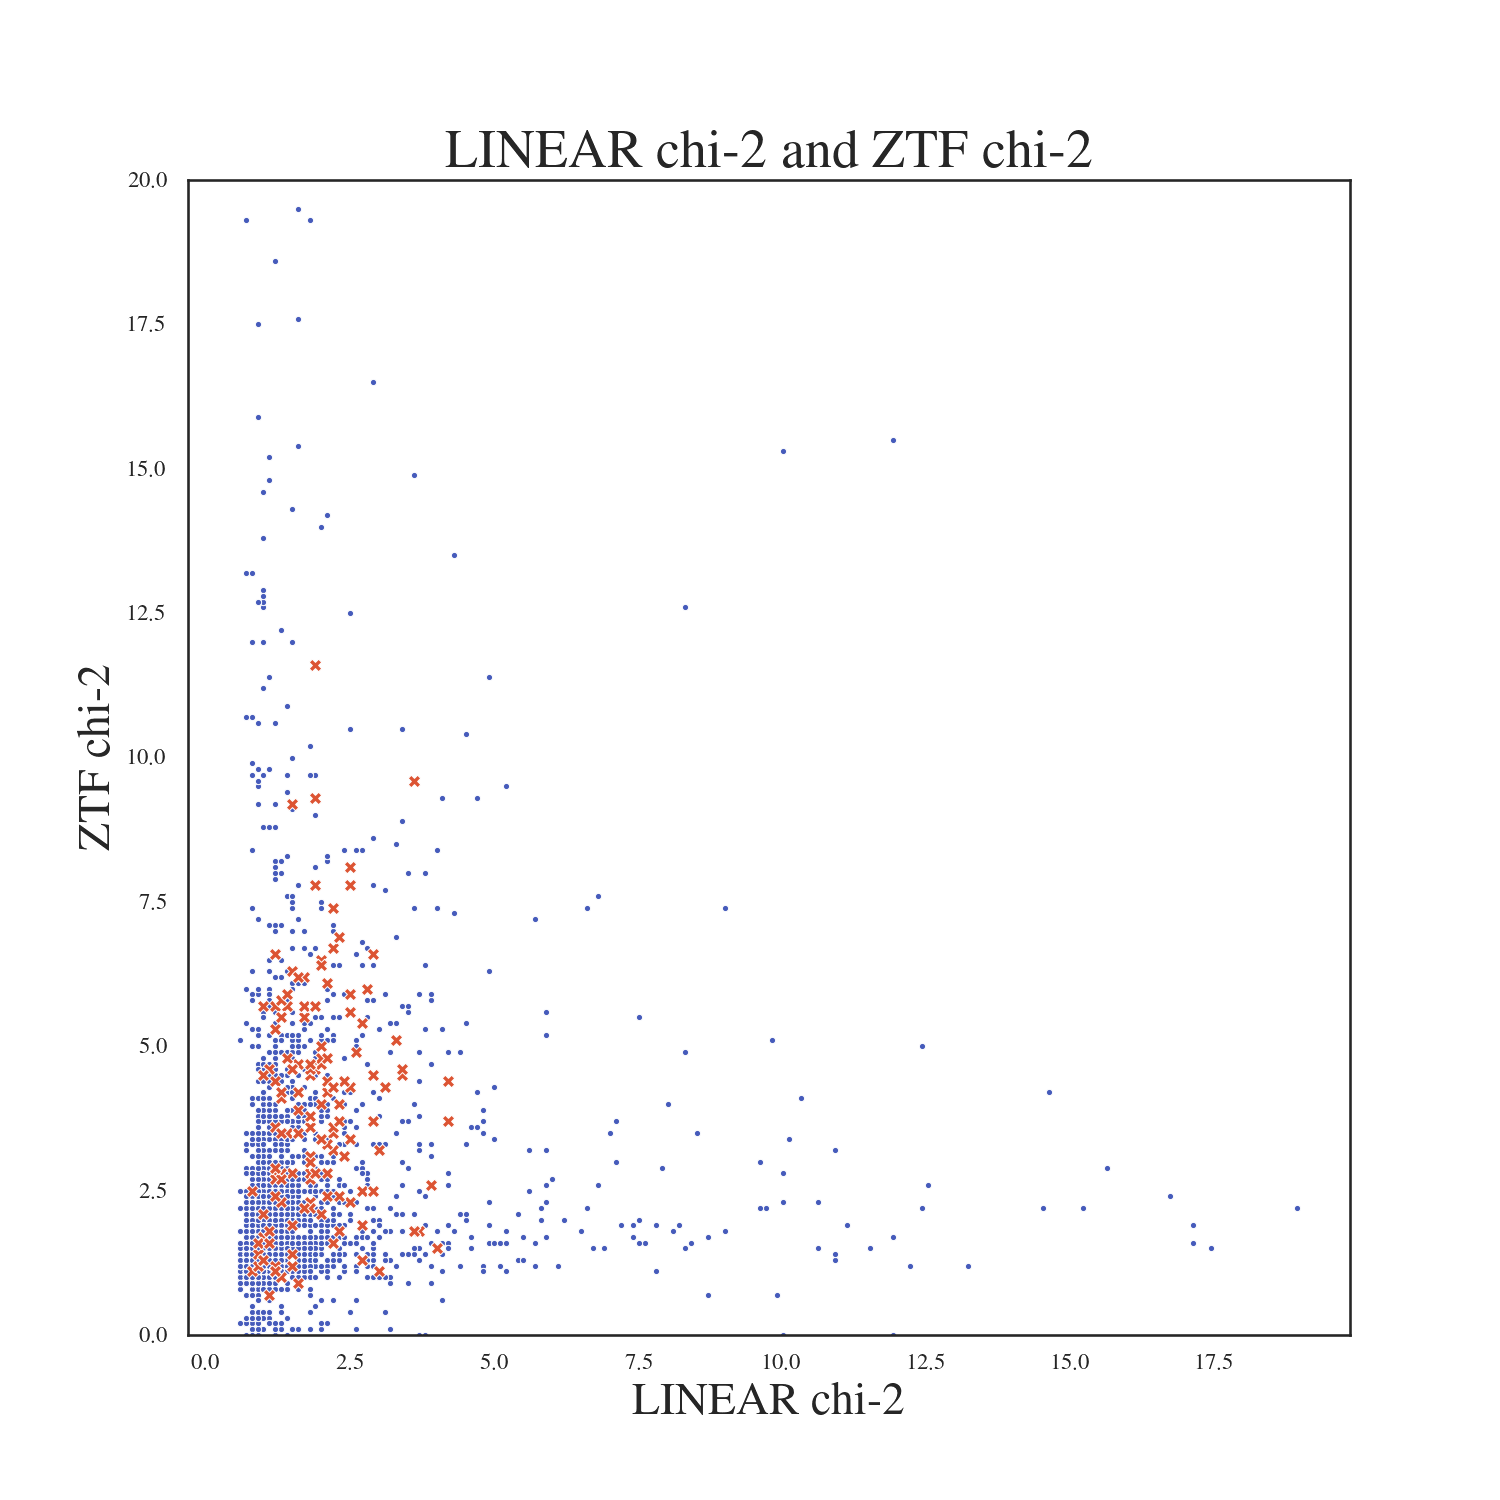
\includegraphics{chi_scatter.png}}
\caption{$\chi^2$ values for LINEAR and ZTF, where blue are all RR Lyrae stars and red are Blazhko stars.}
\label{fig:chi2}
\end{figure}

Another important note highlighting the difficulty of finding Blazhko stars is that the absolute Blazhko frequency difference from the main frequency is approximately 0.028 $d^{-1}$. Also, the average period difference between LINEAR and ZTF in Blazhko stars was around 0.0001 days. These minimal differences require precise observations over a long temporal baseline. The distribution of RRab and RRc type RR Lyrae in our sample is representative of other surveys, where 71\% were type RRab and 29\% RRc type.

Finally, we have discovered that in some Blazhko stars, the effect cannot be detected ten years later or beforehand. When comparing LINEAR and ZTF data, some pairs have the effect present in only one dataset and others in both. This finding could mean that the Blazhko effect is not always present and gives us a clue about its mechanism. However, the precision of data is also a factor for consideration. 

\begin{figure*}[ht]
  \centering
  
\includegraphics[width=17cm]{LCplot_7048826.png}
       \caption{Phase 1 of visual analysis of Blazhko candidates.}
       \label{fig:phase1}
  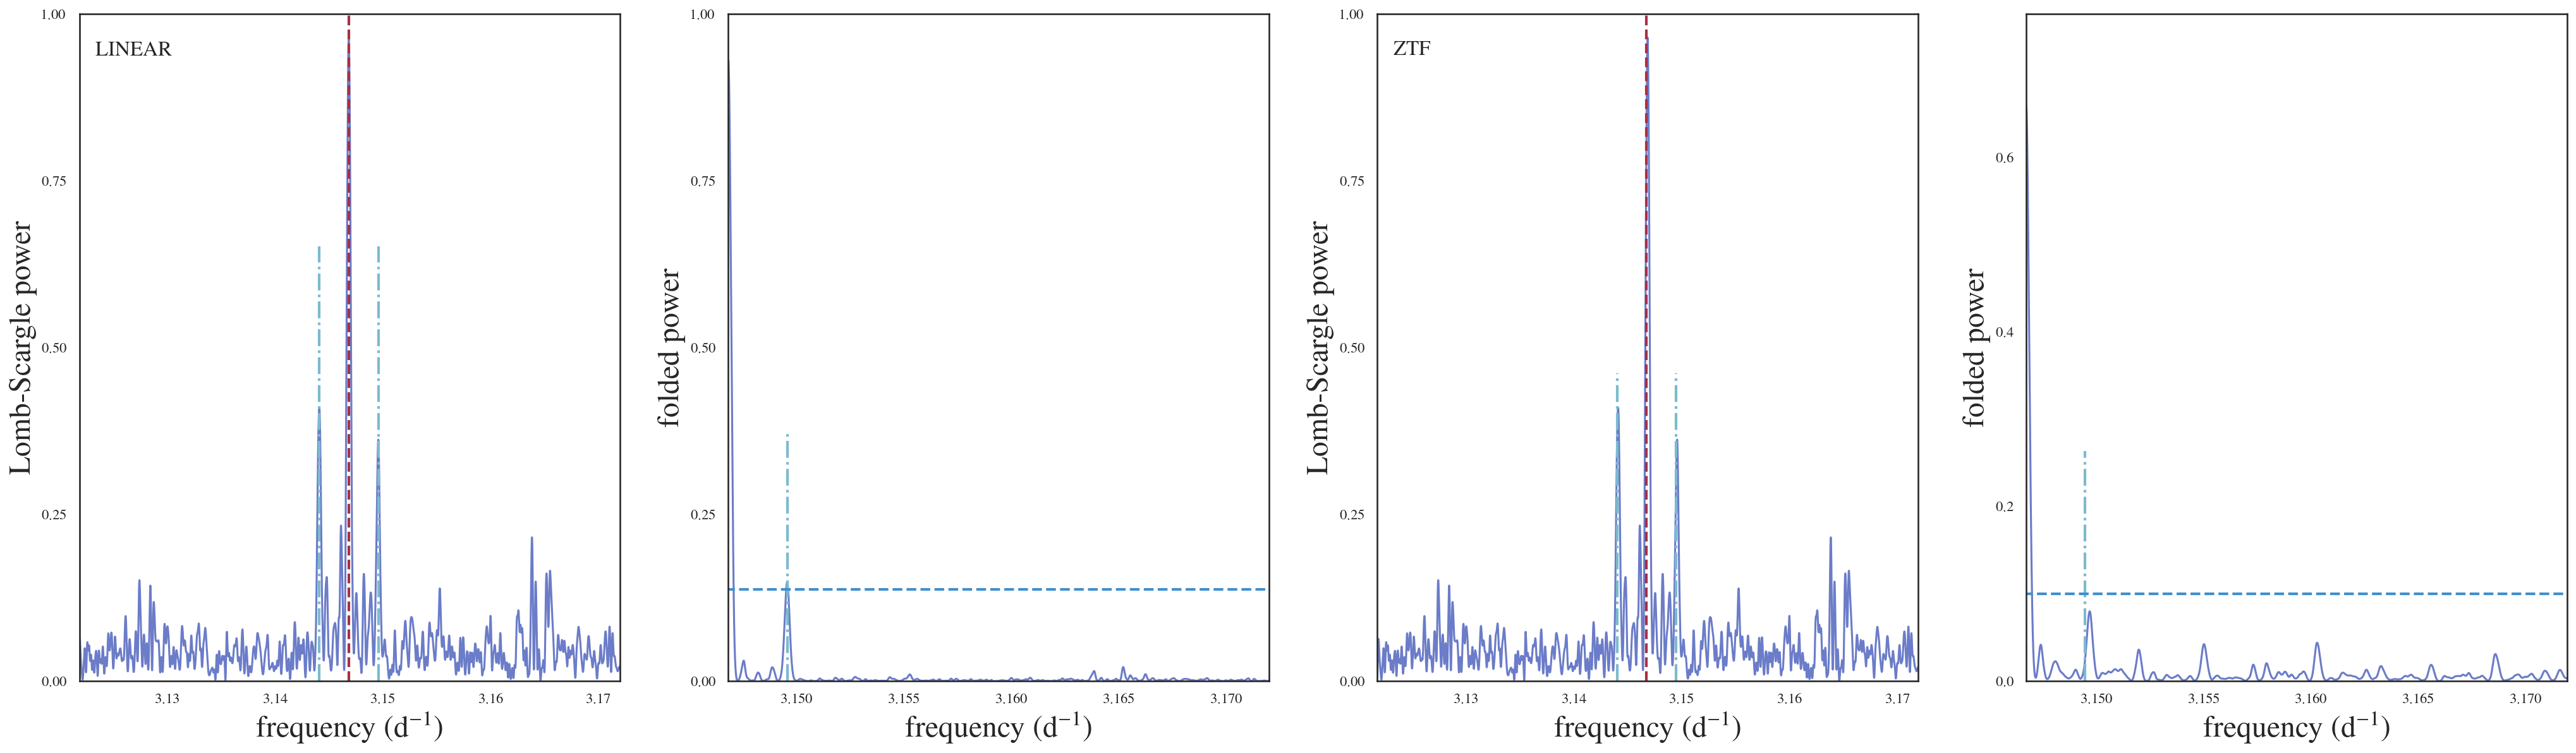
\includegraphics[width=17cm]{periodogram7048826.png}
    \caption{Phase 2 of visual analysis of Blazhko candidates.}
    \label{fig:phase2}

    \centering
       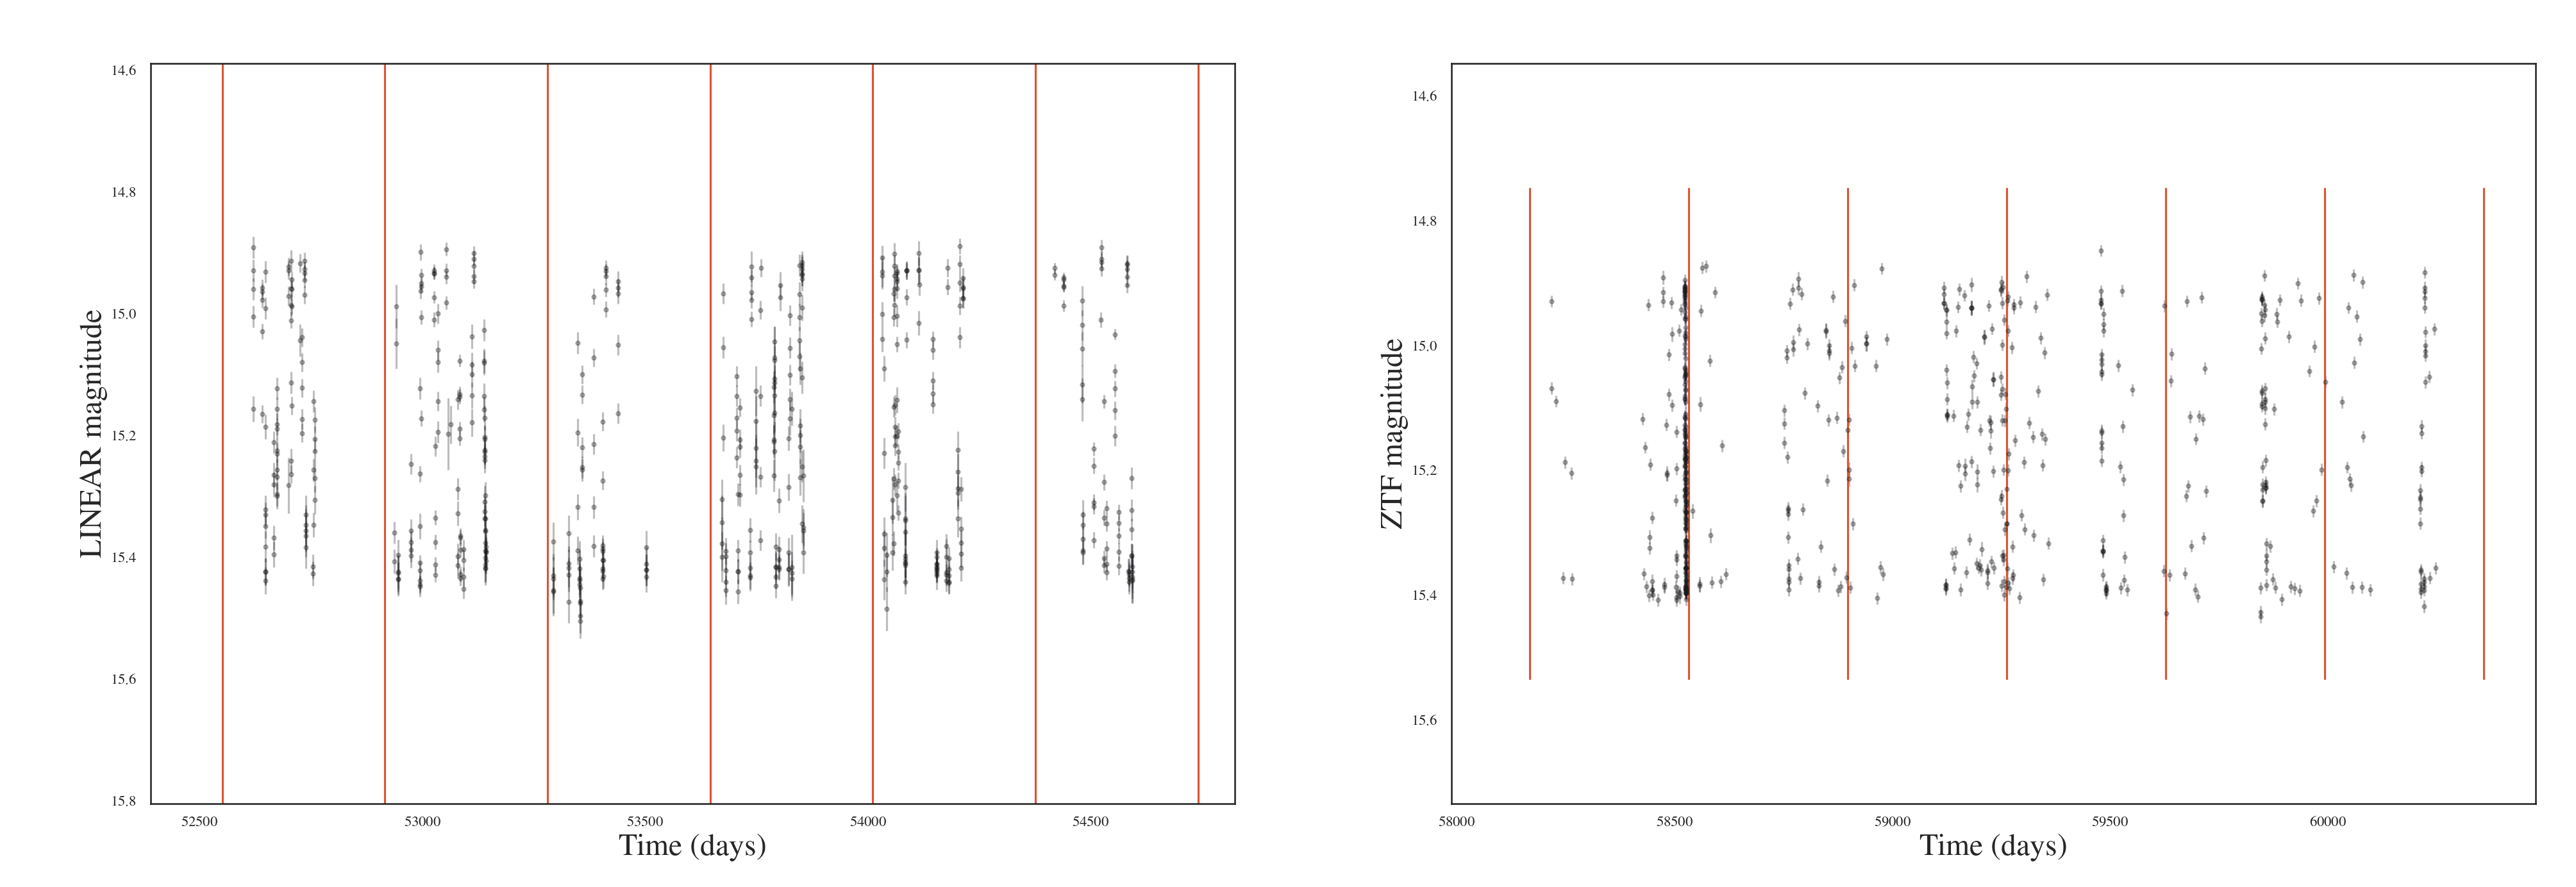
\includegraphics[width=17cm]{season_plot7048826.png}
         \caption{Phase 3 of visual analysis of Blazhko candidates.}
         \label{fig:phase3}
\end{figure*}
\begin{figure*}[ht]
    \centering
    \includegraphics[width=17cm]{LCplotBySeason7048826.png}
      \caption{Phase 4 of visual analysis of Blazhko candidates.}
      \label{fig:phase4}
\end{figure*}

\section{Discussion and Conclusions\label{sec:discussion}}

The reported incidence rates for the Blazhko effect
range from 5\% \citep{2007MNRAS.377.1263S} to 60\% \citep{2014A&A...570A.100S}. For a relatively small sample of
151 stars with Kepler data, a claim has been made that essentially every RR Lyrae star exhibits modulated light curve
\citep{2018A&A...614L...4K}. The difference in Blazhko incidence rates for the two most extensive samples, obtained
by the OGLE-III survey for the Large Magellanic Cloud (LMC, 20\% out of 17,693 stars; \citealt{2009AcA....59....1S}).
Moreover, the Galactic bulge (30\% out of 11,756 stars; \citealt{2011AcA....61....1S}) indicates a possible variation of
the Blazhko incidence rate with underlying stellar population properties. In this work, 4.67\% of the original RR Lyrae dataset are Blazhko stars. Since our sample size is considerable, we conclude that the incidence rate of Blazhko stars in our work is representative and aligns with other works. We theorize that the difference in incidence rates occurs due to varying data precision, the temporal baseline length, and differences in visual or algorithmic analysis.
We also conclude that our algorithm's success rate in finding 136 out of 239 potential Blazhko stars is 57\% . This high number indicates that the algorithm is very successful and can be used and refined further for efficient Blazhko star selection. 

For future research, we would like to explore the final finding and find a connection or a factor that might give rise to a mechanism that explains the Blazhko effect. The project is an excellent example of automatizing the search for Blazhko stars. It can further be improved by training a neural network to replace visual analysis, and our current algorithms can be improved with other models. This work can provide a base for finding more Blazhko stars for the future Vera Rubin observatory. The Legacy Survey of Space and Time (LSST; \citealt{2019ApJ...873..111I}) will be an excellent survey for studying Blazhko effect
\citep{2022ApJS..258....4H} because it will have both a long temporal
baseline (10 years) and a large number of observations per object
(nominally 825; LSST Science Requirements Document\footnote{Available as ls.st/srd}). We hope this work helped in the ongoing research on the Blazhko effect. 

\begin{acknowledgements}
  LINEAR and ZTF acknowledgements.
  Thanks to Mathew Graham for {\it ztfquery} example.
  \v{Z}.I. acknowledges funding by the Fulbright Foundation 
  and thanks the Ru\d er Bo\v{s}kovi\'{c} Institute for 
  hospitality.
  \end{acknowledgements}

\newpage
\bibliographystyle{aa} % style aa.bst
\bibliography{references} % your references Yourfile.bib

\onecolumn
\begin{appendix}

\section{Full table of results}
Here we present all the confirmed Blazhko stars with their LINEAR IDs, equatorial coordinates, and calculated periods and $\chi^2$ values.
\begin{longtable}{lrrrrrrr}
    \toprule
    LINEAR ID & RA & DEC & LINEAR period & ZTF period & LINEAR chi-2 & ZTF chi-2 \\
        \midrule
    \endfirsthead
    
    \toprule
    LINEAR ID & RA & DEC & LINEAR period & ZTF period & LINEAR chi-2 & ZTF chi-2 \\
    \midrule
    \endhead
    
    \midrule
    \endfoot
    
    \bottomrule
    \endlastfoot
    
    523832 & 207.529404 & 33.706001 & 0.372376 & 0.372384 & 1.20 & 1.10 \\
1240665 & 206.202469 & 34.058662 & 0.632528 & 0.632522 & 3.00 & 1.10 \\
1736308 & 206.096115 & 36.648674 & 0.555848 & 0.555843 & 1.30 & 1.00 \\
2669011 & 206.229523 & 38.758453 & 0.591153 & 0.591151 & 1.10 & 0.70 \\
2742032 & 207.355225 & 39.589951 & 0.629676 & 0.629692 & 0.90 & 1.40 \\
2812086 & 206.805511 & 40.859066 & 0.646015 & 0.646000 & 3.00 & 3.20 \\
3507643 & 206.557358 & 39.536449 & 0.801141 & 0.801132 & 1.60 & 0.90 \\
5931160 & 207.177231 & 41.918797 & 0.664700 & 0.664708 & 0.80 & 1.10 \\
6665721 & 206.020233 & 41.646141 & 0.643318 & 0.643325 & 1.00 & 1.70 \\
17185566 & 206.387268 & 43.314617 & 0.614160 & 0.614169 & 1.50 & 1.90 \\
22828215 & 206.657028 & 43.543236 & 0.574536 & 0.574535 & 1.50 & 1.40 \\
29848 & 206.917358 & 44.971054 & 0.557020 & 0.557040 & 1.40 & 3.50 \\
158779 & 207.772202 & 45.916824 & 0.609207 & 0.609189 & 1.60 & 3.90 \\
263541 & 207.172470 & 45.713154 & 0.558218 & 0.558221 & 2.90 & 6.60 \\
514883 & 206.594757 & 46.482040 & 0.557723 & 0.557737 & 1.70 & 5.50 \\
737951 & 206.435547 & 45.881615 & 0.357023 & 0.357023 & 2.20 & 6.70 \\
810169 & 169.297485 & 6.265203 & 0.465185 & 0.465212 & 2.10 & 2.80 \\
924301 & 169.713531 & 6.963072 & 0.507503 & 0.507440 & 1.90 & 9.30 \\
1092244 & 207.060974 & 5.649392 & 0.649496 & 0.649558 & 1.20 & 3.60 \\
1244554 & 206.944962 & 5.346962 & 0.536875 & 0.536962 & 1.80 & 2.30 \\
1307948 & 206.223587 & 6.741248 & 0.527474 & 0.527415 & 1.80 & 4.50 \\
1332201 & 207.992432 & -4.603579 & 0.580711 & 0.580731 & 1.60 & 4.20 \\
1390653 & 207.220245 & -3.214271 & 0.521867 & 0.521871 & 1.30 & 4.10 \\
1435279 & 207.824600 & -3.712567 & 0.381858 & 0.381860 & 2.10 & 4.20 \\
1448299 & 206.582916 & 51.406654 & 0.606912 & 0.606940 & 2.70 & 5.40 \\
1593736 & 169.096771 & 5.428976 & 0.592628 & 0.592650 & 1.20 & 5.70 \\
1748058 & 207.353790 & 53.020401 & 0.310237 & 0.310176 & 1.40 & 5.70 \\
1857382 & 206.026001 & 56.421604 & 0.566428 & 0.566407 & 2.70 & 2.50 \\
1882354 & 207.117645 & 56.313797 & 0.695061 & 0.695029 & 1.50 & 2.80 \\
2041979 & 206.848053 & 55.248009 & 0.653694 & 0.653639 & 1.20 & 5.30 \\
2075949 & 207.733643 & 62.320267 & 0.477806 & 0.477666 & 1.60 & 4.70 \\
2117028 & 207.188278 & 61.978554 & 0.591245 & 0.591243 & 2.20 & 3.50 \\
2122319 & 206.210190 & 62.778843 & 0.359422 & 0.359424 & 2.10 & 6.10 \\
2229607 & 207.042603 & 65.877083 & 0.575179 & 0.575211 & 1.20 & 4.40 \\
2243683 & 206.780823 & 8.893113 & 0.579777 & 0.579803 & 3.10 & 4.30 \\
2248787 & 206.407776 & 7.914382 & 0.563528 & 0.563539 & 2.10 & 2.40 \\
2334384 & 206.454544 & 7.380644 & 0.555341 & 0.555333 & 2.00 & 6.50 \\
2397296 & 168.680649 & 51.998081 & 0.488814 & 0.488836 & 1.20 & 6.60 \\
2414841 & 206.101624 & 7.666218 & 0.559611 & 0.559592 & 1.70 & 5.70 \\
2455568 & 168.211075 & 51.534416 & 0.594119 & 0.594092 & 2.00 & 2.10 \\
2612592 & 207.693237 & -5.975360 & 0.571562 & 0.571543 & 1.30 & 2.80 \\
2653982 & 168.135025 & 51.014339 & 0.607082 & 0.607110 & 1.00 & 2.10 \\
2766997 & 207.782440 & -7.099904 & 0.289881 & 0.289943 & 1.80 & 3.60 \\
2892940 & 209.495773 & 2.587467 & 0.539855 & 0.539896 & 1.30 & 4.20 \\
3036295 & 209.338211 & 2.393512 & 0.629705 & 0.629714 & 1.80 & 2.20 \\
3140139 & 208.758163 & -0.100046 & 0.304590 & 0.304585 & 2.50 & 5.60 \\
3183285 & 208.391159 & 0.479103 & 0.349653 & 0.349664 & 1.20 & 2.80 \\
3196582 & 208.521881 & 0.740297 & 0.268017 & 0.268018 & 2.50 & 3.40 \\
3196780 & 169.384384 & 53.303658 & 0.504148 & 0.504199 & 2.20 & 3.20 \\
3294319 & 169.550766 & 53.459976 & 0.555460 & 0.555473 & 1.90 & 4.70 \\
3437725 & 208.845749 & 12.514306 & 0.542457 & 0.542478 & 1.50 & 6.30 \\
3591037 & 208.146072 & 14.167974 & 0.558643 & 0.558609 & 1.30 & 3.50 \\
3941776 & 209.073120 & 13.401526 & 0.532222 & 0.532209 & 2.80 & 6.00 \\
4101289 & 209.351425 & 13.537904 & 0.379225 & 0.379250 & 1.20 & 2.70 \\
4586691 & 208.326218 & 15.475822 & 0.621459 & 0.621446 & 2.00 & 3.40 \\
4804945 & 209.674210 & 16.421736 & 0.556172 & 0.556217 & 2.50 & 7.80 \\
5421989 & 208.014435 & 18.561077 & 0.534510 & 0.534527 & 0.80 & 2.50 \\
6582265 & 209.421219 & 17.441139 & 0.691751 & 0.691749 & 2.90 & 3.70 \\
6651516 & 208.909760 & 17.881287 & 0.308488 & 0.308496 & 1.30 & 5.80 \\
6819457 & 209.491974 & 20.296762 & 0.436282 & 0.436265 & 3.60 & 9.60 \\
6883239 & 208.333481 & 19.276327 & 0.563711 & 0.563712 & 2.90 & 2.50 \\
6967017 & 208.406662 & 21.846382 & 0.529691 & 0.529677 & 2.30 & 6.90 \\
7048826 & 208.492981 & 22.591896 & 0.317781 & 0.317790 & 1.40 & 5.90 \\
7254801 & 209.648148 & 22.561989 & 0.561133 & 0.561071 & 1.30 & 5.50 \\
7279621 & 208.915436 & 24.833937 & 0.415469 & 0.415467 & 1.90 & 4.60 \\
7283275 & 208.409698 & 26.350325 & 0.543342 & 0.543331 & 2.20 & 3.60 \\
7344401 & 209.188583 & 26.111385 & 0.330201 & 0.330226 & 1.80 & 2.70 \\
7580734 & 209.349243 & 26.322409 & 0.314956 & 0.314957 & 2.00 & 4.00 \\
7657340 & 208.098282 & 27.700201 & 0.495480 & 0.495493 & 2.30 & 4.00 \\
7811366 & 208.457687 & 30.868412 & 0.489523 & 0.489521 & 2.00 & 4.70 \\
7827663 & 208.047531 & 30.799057 & 0.390832 & 0.390832 & 3.40 & 4.50 \\
7846640 & 209.106400 & 4.330462 & 0.551495 & 0.551518 & 1.50 & 9.20 \\
8222011 & 209.258850 & 3.100914 & 0.350920 & 0.350914 & 2.00 & 4.80 \\
8311517 & 208.212936 & 4.452833 & 0.523354 & 0.523359 & 1.80 & 3.60 \\
8331094 & 208.446945 & 3.969552 & 0.267543 & 0.267549 & 2.10 & 3.30 \\
8343291 & 208.919601 & -2.689821 & 0.569785 & 0.569791 & 3.30 & 5.10 \\
9063194 & 169.357468 & 57.331566 & 0.575781 & 0.575760 & 2.40 & 3.10 \\
9236215 & 209.009872 & -1.607280 & 0.352570 & 0.352572 & 1.80 & 2.80 \\
9449335 & 209.488937 & -2.928472 & 0.475720 & 0.475695 & 2.00 & 5.00 \\
9532981 & 168.695602 & 60.104759 & 0.591000 & 0.591042 & 1.70 & 6.20 \\
9918809 & 209.255295 & -2.089725 & 0.479460 & 0.479509 & 1.90 & 11.60 \\
9968431 & 209.717804 & -2.437493 & 0.302266 & 0.302211 & 1.70 & 2.20 \\
9979905 & 208.905365 & 31.572962 & 0.338739 & 0.338739 & 2.50 & 2.30 \\
10030349 & 209.547668 & 32.537975 & 0.545073 & 0.545074 & 2.10 & 4.40 \\
10260828 & 208.891602 & 32.249817 & 0.380655 & 0.380643 & 2.20 & 7.40 \\
10814742 & 209.570526 & 31.039347 & 0.462687 & 0.462683 & 2.50 & 4.30 \\
11215595 & 208.180191 & 33.574619 & 0.546960 & 0.546943 & 1.30 & 2.30 \\
16991760 & 209.105652 & 33.977589 & 0.549098 & 0.549096 & 2.90 & 3.70 \\
17247918 & 169.489120 & 59.391106 & 0.481867 & 0.481865 & 1.80 & 4.60 \\
17275627 & 208.806717 & 33.957424 & 0.537775 & 0.537771 & 2.10 & 4.80 \\
17302403 & 209.807205 & 35.285717 & 0.488261 & 0.488343 & 2.00 & 6.40 \\
17544856 & 208.748581 & 36.859768 & 0.614297 & 0.614296 & 2.00 & 3.40 \\
19775800 & 208.958618 & 36.484657 & 0.310856 & 0.310867 & 1.30 & 2.70 \\
21488669 & 209.334930 & 37.248749 & 0.501644 & 0.501661 & 1.90 & 5.70 \\
21556651 & 208.269577 & 38.000725 & 0.614826 & 0.614808 & 1.80 & 3.10 \\
21619184 & 208.125366 & 37.095997 & 0.557343 & 0.557320 & 2.30 & 3.70 \\
21806402 & 208.151657 & 39.543987 & 0.592081 & 0.592104 & 1.60 & 6.20 \\
21874209 & 209.602371 & 40.245346 & 0.611295 & 0.611286 & 2.50 & 5.90 \\
21967825 & 209.202347 & 39.452202 & 0.540607 & 0.540600 & 1.80 & 4.70 \\
22244513 & 208.742203 & 41.386112 & 0.604149 & 0.604077 & 2.50 & 8.10 \\
22319996 & 209.734711 & 42.773571 & 0.479505 & 0.479495 & 2.60 & 4.90 \\
22518636 & 208.239105 & 41.299026 & 0.283996 & 0.283998 & 1.80 & 3.00 \\
22959674 & 209.018127 & 41.835575 & 0.405333 & 0.405409 & 1.80 & 3.80 \\
22980793 & 208.105713 & 44.400867 & 0.540348 & 0.540353 & 1.90 & 2.80 \\
23135759 & 209.604721 & 45.746510 & 0.402730 & 0.402732 & 4.20 & 4.40 \\
23148883 & 209.446594 & 45.757584 & 0.390130 & 0.390124 & 1.40 & 4.80 \\
23184808 & 208.547745 & 47.825001 & 0.338821 & 0.338888 & 1.00 & 5.70 \\
23193507 & 208.703445 & 49.226929 & 0.473158 & 0.473174 & 3.40 & 4.60 \\
23653629 & 209.116013 & 50.653641 & 0.442052 & 0.442055 & 2.40 & 4.40 \\
24019356 & 208.649506 & 50.454273 & 0.517473 & 0.517460 & 1.50 & 4.60 \\
24020106 & 209.853088 & 5.836339 & 0.542397 & 0.542396 & 2.90 & 4.50 \\
24216004 & 209.385406 & 6.251467 & 0.382077 & 0.381912 & 1.90 & 7.80 \\
880588 & 208.532242 & 6.762656 & 0.600138 & 0.600134 & 1.20 & 2.40 \\
1212611 & 208.592422 & 6.144436 & 0.630896 & 0.630893 & 0.90 & 1.20 \\
1876491 & 209.131027 & 5.983884 & 0.760128 & 0.760123 & 1.20 & 1.20 \\
3048546 & 209.125137 & -4.194337 & 0.656287 & 0.656293 & 1.00 & 1.30 \\
5272753 & 208.115189 & -4.847239 & 0.485827 & 0.485831 & 0.90 & 1.60 \\
8610884 & 208.744736 & -4.852155 & 0.592421 & 0.592429 & 2.20 & 4.30 \\
8907563 & 209.521454 & -3.322183 & 0.513164 & 0.513164 & 1.10 & 4.60 \\
9852554 & 208.390961 & -4.619442 & 0.651339 & 0.651367 & 1.00 & 4.50 \\
9961135 & 209.178848 & 52.903030 & 0.590896 & 0.590891 & 1.10 & 1.80 \\
10503746 & 208.417831 & 54.266953 & 0.573563 & 0.573570 & 2.70 & 1.90 \\
21948290 & 209.862518 & 56.455978 & 0.511127 & 0.511115 & 2.30 & 2.40 \\
23596342 & 209.988663 & 56.828396 & 0.602841 & 0.602846 & 1.20 & 2.90 \\
23898397 & 121.150764 & 42.483574 & 0.563018 & 0.562989 & 1.60 & 3.50 \\
1882088 & 208.323578 & 58.245502 & 0.315984 & 0.316041 & 4.00 & 1.50 \\
2936953 & 208.351578 & 57.226521 & 0.328746 & 0.328733 & 2.70 & 1.30 \\
3219035 & 209.858856 & 60.601982 & 0.326746 & 0.326509 & 3.90 & 2.60 \\
4320492 & 168.062149 & 65.801857 & 0.361005 & 0.360942 & 3.70 & 1.80 \\
8036191 & 208.732498 & 59.448402 & 0.363860 & 0.363893 & 2.20 & 1.60 \\
10420063 & 209.945786 & 61.264187 & 0.487395 & 0.487394 & 4.20 & 3.70 \\
10662468 & 209.124405 & 61.076996 & 0.445180 & 0.445167 & 3.60 & 1.80 \\
21688272 & 209.311371 & 62.800976 & 0.304803 & 0.304790 & 2.30 & 1.80 \\
2714034 & 168.354202 & 65.678604 & 0.610868 & 0.610800 & 1.50 & 1.20 \\
5592590 & 208.440872 & 65.857277 & 0.346945 & 0.346980 & 1.20 & 1.10 \\
8799313 & 208.821136 & 7.846983 & 0.327560 & 0.327542 & 1.10 & 1.60 \\
\bottomrule
\end{longtable}
    

\end{appendix}
\twocolumn
\end{document}